%\documentclass{beamer}
\documentclass[usenames,dvipsnames]{beamer}
\setbeamertemplate{navigation symbols}{}  % remove navigation symbols

%\usepackage{beamerthemesplit}

%\usetheme{default}
\usetheme{Pittsburgh}

%\usecolortheme{beaver}
\usecolortheme{spruce}

% color theme: beaver = red
% color theme: spruce = green
% 
% Theme: Frankfurt 
% Theme: Malmoe
% Theme: Rochester
% 
% Theme: Szeged, Color Theme: beaver

\setbeamersize{text margin left=0ex, text margin right=0ex}


\usepackage{color}
%\usepackage[usenames,dvipsnames]{color}  % see http://en.wikibooks.org/wiki/LaTeX/Colors
\usepackage[latin1]{inputenc}
\usepackage{enumerate}

\usepackage{graphicx}
\usepackage{amsmath}
\usepackage{amssymb}
\usepackage{url}
\usepackage{mathtools}
\usepackage{xspace}
\usepackage{multirow}
\usepackage{booktabs}
\usepackage{algorithmic}
\usepackage{algorithm}
\usepackage{xfrac}
\usepackage{fancyvrb}
\usepackage{adjustbox}

\usepackage[british]{babel}
\usepackage[none]{hyphenat}
\sloppy

\usepackage{palatino}     % changes the default sans serif font
\usepackage{inconsolata}  % changes the default typewriter font

% disable ligatures such as "fi" being joined into one symbol
\usepackage{microtype}
\DisableLigatures[f]{encoding = *, family = * }

\def\_{{\tt\char95}}

\graphicspath{{./}{./figures/}}

\DeclareMathOperator*{\argmin}{argmin}

\def\Vec#1{{\boldsymbol{#1}}}
\def\Mat#1{{\boldsymbol{#1}}}
\def\TODO#1{{\color{red}{\bf [TODO:} {\it{#1}}{\bf ]}}}
\def\NOTE#1{{\bf [NOTE:} {\it\color{blue}{#1}}{\bf ]}.}
\def\CHK#1{{\bf [CHECK:} {\it\color{red} {#1}}{\bf ]}.}
\def\eg{eg.\xspace}
\def\ie{ie.\xspace}
\def\etal{et~al.\xspace}

\renewcommand{\baselinestretch}{1.2}\small\normalsize


% \title{A Tiny Example}
% \author{Andrew Mertz and William Slough}
% \date{June 15, 2005}
\begin{document}


\begin{frame}
% \frametitle{~}
\textcolor{ForestGreen}{\hrule}
\textcolor{ForestGreen}{\hrule}
\textcolor{ForestGreen}{\hrule}
\centerline{~}
\centerline{\Large\bf An Open Source C++ Implementation of}
\centerline{\Large\bf Multi-Threaded Gaussian~Mixture~Models}
\centerline{\Large\bf k-Means and Expectation Maximisation}
\vspace{-1ex}
\textcolor{ForestGreen}{\hrule}
\textcolor{ForestGreen}{\hrule}
\textcolor{ForestGreen}{\hrule}
\centerline{~}
\centerline{~}
\centerline{\large Conrad Sanderson ~and~ Ryan Curtin}
\centerline{~}

\begin{center}
\begin{minipage}{1\textwidth}
\centering

\begin{minipage}{0.24\textwidth}
% centering deliberately omitted for this cell
\centering

\includegraphics[height=1.25cm]{data61_logo_scaled_crop.png}
\end{minipage}
\begin{minipage}{0.35\textwidth}
\centering

\includegraphics[height=1.10cm]{UQ_logo.pdf}
\end{minipage}
\begin{minipage}{0.17\textwidth}
\centering

\includegraphics[height=1.25cm]{symantec_logo.pdf}
\end{minipage}
\begin{minipage}{0.17\textwidth}
\centering

\includegraphics[height=1.25cm]{arroyo_logo.png}
\end{minipage}

\end{minipage}
\end{center}

\centerline{~}


\begin{center}
\begin{minipage}{0.5\textwidth}
{\large\textcolor{red}{\small\texttt{Conrad~-~\href{http://conradsanderson.id.au}{http://conradsanderson.id.au}}}}\\
{\large\textcolor{red}{\small\texttt{Ryan~~~-~\href{http://ratml.org}{http://ratml.org}}}}
\end{minipage}
\end{center}

\end{frame}

%\footnotesize
%\fontsize{8}{9}\selectfont

\makeatletter
\renewcommand\normalsize{\@setfontsize\normalsize{8.5pt}{9.5pt}}
\normalsize  
\makeatother

\makeatletter
\renewcommand\small{\@setfontsize\normalsize{8.5pt}{9.5pt}}
\normalsize  
\makeatother


\begin{frame}
\frametitle{Background / 1}

\begin{enumerate}[{~~$\boldsymbol{\bullet}$}]

\item {\bf Gaussian Mixture Models (GMMs)} are used for approximating arbitrary distributions
\vspace{1ex}

\item Distribution of samples (vectors) is modelled as:

\begin{equation*}
  p(\Vec{x} | \lambda) = \sum\nolimits_{g=1}^{N_G} w_g ~ {{\mathcal{N}}}( \Vec{x} | \Vec{\mu}_g, \Mat{\Sigma}_g )
\end{equation*}%
%
where:

\begin{enumerate}[{$\boldsymbol{\rightarrow}$}]
\renewcommand{\itemsep}{0.9ex}

\item $\Vec{x}$ is a $D$-dimensional vector
\item $\lambda = \{ w_g, \Vec{\mu}_g, \Mat{\Sigma}_g \}_{g=1}^{N_G}$ is the parameter set
\item  $w_g$ is the weight for component $g$, with constraints $\sum\nolimits_{g=1}^{N_G} w_g = 1$, $w_g \geq 0$

\item \scalebox{0.93}{${{\mathcal{N}}}( \Vec{x} | \Vec{\mu}, \Mat{\Sigma})$ is a $D$-dimensional Gaussian density function with mean $\Vec{\mu}$ and covariance matrix $\Mat{\Sigma}$:}

\begin{equation*}
  {{\mathcal{N}}}( \Vec{x} | \Vec{\mu}, \Mat{\Sigma} )  = 
  \frac{1}{ (2\pi)^{\frac{D}{2}} | \Mat{\Sigma}|^{\frac{1}{2}} }
  \exp \left[ -\frac{1}{2} (\Vec{x}-\Vec{\mu})^\top \Mat{\Sigma}^{-1} (\Vec{x}-\Vec{\mu}) \right]
  \label{eqn:gaussian}
\end{equation*}%

\end{enumerate}

\item {\bf Many use cases}

\begin{enumerate}[{$\boldsymbol{\rightarrow}$}]
\renewcommand{\itemsep}{0.9ex}
\item signal processing, computer vision, machine learning, finance, even deep learning!
\vspace{0.5ex}
\end{enumerate}

\end{enumerate}
\end{frame}

%
%
%

\begin{frame}
\frametitle{Background / 2}

\begin{enumerate}[{~~$\boldsymbol{\bullet}$}]

\item Many publically accessible implementations are available, {\bf but have problems:}

\begin{enumerate}[{$\boldsymbol{\rightarrow}$}]
\renewcommand{\itemsep}{0.9ex}
\item 
{\bf restrictive license}\\
eg.~can't use in commercial products

\item
{\bf serial execution}\\
doesn't take advantage of multi-core systems

\item
{\bf naive implementation} of training algorithms\\
numerically unstable

\item
{\bf poor interface} for use of models and modifying model parameters

\item
implemented in {\bf outdated} and {\bf error-prone} languages\\
eg.~C\\
fast to execute, good for embedding, but absolutely horrible for development

\item
implemented in {\bf non-embeddable} languages\\
eg.~Python, Matlab, ...\\
good for prototyping, bad for embedding into products or larger software

\end{enumerate}

\end{enumerate}
\end{frame}

%
%
%

\begin{frame}
\frametitle{Overview}

\begin{enumerate}[{~~$\boldsymbol{\bullet}$}]

\item We provide an open source implementation which avoids the problems

\begin{enumerate}[{$\boldsymbol{\rightarrow}$}]
\renewcommand{\itemsep}{1ex}
\item 
{\bf permissive open source license}\\
- Apache 2.0\\
- commercial software and products DO NOT need to release their source code\\
- better than BSD license: provides explicit patent grants

\item
{\bf multi-core execution}\\
- the more cores, the faster it runs\\
- internally uses a MapReduce-like approach

\item
training algorithms use elaborate methods to {\bf promote numerical stability}

\item
{\bf flexible interface} to trained models

\item
implemented as {\bf encapsulated classes} in {\bf modern C++}\\
- provides nice abstractions to make software development easier

\item
can be easily {\bf embedded} into products or larger software\\

\item
{\bf battle tested}\\
successfully used in many projects

\end{enumerate}

\end{enumerate}
\end{frame}

%
%
%

\begin{frame}
\frametitle{Single-Threaded EM Training}

\begin{enumerate}[{~~$\boldsymbol{\bullet}$}]
\renewcommand{\itemsep}{1ex}

\item Each GMM is parameterised with $\lambda = \{ w_g, \Vec{\mu}_g, \Mat{\Sigma}_g \}_{g=1}^{N_G}$

\item Given training data $X=\{\Vec{x}_i\}_{i=1}^{N_V}$, use Expectation-Maximisation (EM) algorithm to find $\lambda$

\item EM iterates such that $p(X|\lambda^{\textrm{new}}) \geq p(X|\lambda^{\textrm{old}})$

\item One iteration of EM, {\bf single threaded}:

\begin{minipage}{1\textwidth}

\begin{minipage}{0.45\textwidth}
\centering
%
\begin{eqnarray*}
  l_{g,i}                  & = & \frac{w_g ~ {{\mathcal{N}}}( \Vec{x}_i | \Vec{\mu}_g, \Mat{\Sigma}_g )}{\sum\nolimits_{k=1}^{N_G} w_k ~ {{\mathcal{N}}}( \Vec{x}_i | \Vec{\mu}_k, \Mat{\Sigma}_k )} \\
  L_g                      & = & \sum\nolimits_{i=1}^{N_V} l_{g,i} \\
  \widehat{w}_g            & = & \frac{L_g}{N_V} \\
  \widehat{\Vec{\mu}}_g    & = & \frac{1}{L_g} \sum\nolimits_{i=1}^{N_V} l_{g,i} ~ \Vec{x}_i \\
  \widehat{\Mat{\Sigma}}_g & = & \frac{1}{L_g} \sum\nolimits_{i=1}^{N_V} l_{g,i} ~ (\Vec{x}_i - \widehat{\Vec{\mu}}_g)(\Vec{x}_i - \widehat{\Vec{\mu}}_g)^\top 
%                          & = &  \frac{1}{L_g} \left[ \sum\nolimits_{i=1}^{N_V} \Vec{x}_i \Vec{x}_i^\top l_{g,i} \right] - \widehat{\Vec{\mu}}_g \widehat{\Vec{\mu}}_g^\top
\end{eqnarray*}
\end{minipage}
~
\begin{minipage}{0.45\textwidth}
\begin{tiny}%
\begin{equation*}
  {{\mathcal{N}}}( \Vec{x} | \Vec{\mu}, \Mat{\Sigma} )  = 
  \frac{1}{ (2\pi)^{\frac{D}{2}} | \Mat{\Sigma}|^{\frac{1}{2}} }
  \exp \left[ -\frac{1}{2} (\Vec{x}-\Vec{\mu})^\top \Mat{\Sigma}^{-1} (\Vec{x}-\Vec{\mu}) \right]
\end{equation*}%
\end{tiny}%
the $\exp(\cdot)$ function is time consuming\\
\scalebox{0.875}{for large $D$, matrix multiplications are time consuming}
%- calculated independently for each $\Vec{x}_i$\\
~\\
~\\
~\\
weighted version of the sample mean\\
~\\
weighted version of the sample covariance\\
~\\
\end{minipage}

\end{minipage}



% \begin{enumerate}[{$\boldsymbol{\rightarrow}$}]
% \renewcommand{\itemsep}{1ex}
% \item 
% \end{enumerate}

\end{enumerate}
\end{frame}

%
%
%

\begin{frame}
\frametitle{Multi-Threaded EM Training}

\vspace{-1ex}
\begin{enumerate}[{~~$\boldsymbol{\bullet}$}]

\item Adapt {\bf MapReduce} framework

\begin{enumerate}[{$\boldsymbol{\rightarrow}$}]
\renewcommand{\itemsep}{0.5ex}
\item {\bf map:~~~~~} split data into {\bf chunks} and farm it out to {\bf separate threads} for processing
\item {\bf reduce:} collect partial results and {\bf combine} to produce the final result
\end{enumerate}
\vspace{0.5ex}

\item
Rewrite $\widehat{\Mat{\Sigma}}_g$ to allow partial processing:
%{$\widehat{\Mat{\Sigma}}_g = \frac{1}{L_g} \left[ \sum\nolimits_{i=1}^{N_V} l_{g,i} ~ \Vec{x}_i^{~} \Vec{x}_i^\top  \right] - \widehat{\Vec{\mu}}_g^{~} \widehat{\Vec{\mu}}_g^\top$}
%\vspace{1ex}
%\vspace{-1.5ex}
\begin{scriptsize}%
\begin{equation*}
\widehat{\Mat{\Sigma}}_g
~=~ \left\{ \frac{1}{L_g} \sum\nolimits_{i=1}^{N_V} l_{g,i} ~ (\Vec{x}_i - \widehat{\Vec{\mu}}_g)(\Vec{x}_i - \widehat{\Vec{\mu}}_g)^\top \right\}
~=~ \left\{ \frac{1}{L_g} \left[ \sum\nolimits_{i=1}^{N_V} l_{g,i} ~ \Vec{x}_i^{~} \Vec{x}_i^\top  \right] - \widehat{\Vec{\mu}}_g^{~} \widehat{\Vec{\mu}}_g^\top \right\}
\end{equation*}%
\end{scriptsize}
\vspace{-1ex}

\item {\bf Partial} results for thread $t$:
%
\vspace{-3.5ex}
\begin{scriptsize}%
\begin{eqnarray*}
  \widetilde{L}_g^{[t]}            & = & \sum\nolimits_{j = i^{[t]}_{\textrm{start}}}^{i^{[t]}_{\textrm{end}}} l_{g,j}                             \\
  \widetilde{\Vec{\mu}}_g^{[t]}    & = & \sum\nolimits_{j = i^{[t]}_{\textrm{start}}}^{i^{[t]}_{\textrm{end}}} l_{g,j} ~ \Vec{x}_j                 \\
  \widetilde{\Mat{\Sigma}}_g^{[t]} & = & \sum\nolimits_{j = i^{[t]}_{\textrm{start}}}^{i^{[t]}_{\textrm{end}}} l_{g,j} ~ \Vec{x}_j^{~} \Vec{x}_j^\top
\end{eqnarray*}%
\end{scriptsize}
\vspace{-2ex}

\item Threads are executed in {\bf parallel}
\vspace{1ex}

\item {\bf Combine} partial results:
%
\begin{scriptsize}%
\vspace{-3.5ex}
\begin{eqnarray*}
  L_g                      & = & \sum\nolimits_{t=1}^{N_T} \widetilde{L}_g^{[t]} \\
  \widehat{\Vec{\mu}}_g    & = & \frac{1}{L_g} \sum\nolimits_{t=1}^{N_T} \widetilde{\Vec{\mu}}_g^{[t]} \\
  \widehat{\Mat{\Sigma}}_g & = & \frac{1}{L_g} \sum\nolimits_{t=1}^{N_T} \widetilde{\Mat{\Sigma}}_g^{[t]} - \widehat{\Vec{\mu}}_g^{~} \widehat{\Vec{\mu}}_g^\top
\end{eqnarray*}%
\end{scriptsize}



\end{enumerate}
\end{frame}
%
%
%

\begin{frame}
\frametitle{Improving Initial k-Means Estimate}

\begin{enumerate}[{~~$\boldsymbol{\bullet}$}]

\item
To speed up training, {\bf starting point} for EM is typically provided by \textbf{\textit{k}-means}
\vspace{0.5ex}

\item
{\it k}-means is essentially a {\bf simplified version} of the EM algorithm for GMMs
\vspace{0.5ex}

\item
Assignment of each sample to a cluster: {\bf soft assignment} vs {\bf hard assignment}
\vspace{0.5ex}

\item
Estimation of model parameters is the same, except $l_{g,i}$ is redefined~as:%

\vspace{-1.5ex}
\begin{minipage}{1\textwidth}
\begin{minipage}{0.5\textwidth}
\begin{equation*}
  l_{g,i} = \left\{
  \begin{array}{ll}
  1, & \mbox{if} ~ g = \argmin\limits_{k=1, \cdots, N_G} \operatorname{dist}(\Vec{\mu}_k, \Vec{x}_i) \\
  0, & \mbox{otherwise}
  \end{array}
  \right.
\end{equation*}%
\end{minipage}
\begin{minipage}{0.5\textwidth}
{$\operatorname{dist}(\Vec{a}, \Vec{b})$} is a distance metric
\end{minipage}
\end{minipage}
\vspace{0.5ex}


\item 
{\bf Multi-threading} is accomplished in the same manner as for normal EM
\vspace{0.5ex}

\item
{\bf Problem:}
\begin{enumerate}[{$\boldsymbol{\rightarrow}$}]
\renewcommand{\itemsep}{0.9ex}

\item
typical and naive choice:  $\operatorname{dist}(\Vec{a}, \Vec{b}) = \| \Vec{a} - \Vec{b} \|^{2}_{2}$   ~~~ (squared Euclidean distance)

\item
large range in one dimension can skew parameter estimates: {\bf bad starting point!}

\end{enumerate}
\vspace{0.5ex}

\item
{\bf Replace} with squared Mahalanobis distance:
%
\begin{equation*}
\operatorname{dist}(\Vec{a}, \Vec{b}) = (\Vec{a} - \Vec{b})^\top \Mat{\Sigma}^{-1}_{\mathrm{global}} (\Vec{a} - \Vec{b})
\end{equation*}

\begin{enumerate}[{$\boldsymbol{\rightarrow}$}]
\renewcommand{\itemsep}{0.9ex}

\item
$\Mat{\Sigma}_{\mathrm{global}}$ = global covariance matrix, estimated from all available training data

\item
to maintain efficiency, $\Mat{\Sigma}_{\mathrm{global}}$ is typically diagonal

\end{enumerate}



\end{enumerate}
\end{frame}

%
%
%

\begin{frame}
\frametitle{Improving Numerical Stability / 1}

\begin{enumerate}[{~~$\boldsymbol{\bullet}$}]

\item {\bf Problem:} floating point representations have necessarily {\bf limited precision}

\end{enumerate}

\begin{minipage}{1\textwidth}
\begin{minipage}{0.5\textwidth}
\begin{enumerate}[{~~$\boldsymbol{\bullet}$}]
\item Direct calculation of ${{\mathcal{N}}}( \Vec{x} | \Vec{\mu}, \Mat{\Sigma} )$ and $p(\Vec{x} | \lambda)$\\
will quickly lead to {\bf numerical underflows} or~{\bf overflows}
\end{enumerate}
\end{minipage}
\vline~
\begin{minipage}{0.45\textwidth}
~\\
\begin{tiny}
${{\mathcal{N}}}( \Vec{x} | \Vec{\mu}, \Mat{\Sigma} ) = \frac{1}{ (2\pi)^{\frac{D}{2}} | \Mat{\Sigma}|^{\frac{1}{2}} } \exp \left[ -\frac{1}{2} (\Vec{x}-\Vec{\mu})^\top \Mat{\Sigma}^{-1} (\Vec{x}-\Vec{\mu}) \right]$\\
\end{tiny}
~\\
$p(\Vec{x} | \lambda) = \sum\nolimits_{g=1}^{N_G} w_g ~ {{\mathcal{N}}}( \Vec{x} | \Vec{\mu}_g, \Mat{\Sigma}_g )$\\
\end{minipage}

\end{minipage}

\begin{enumerate}[{~~$\boldsymbol{\bullet}$}]

\item Use {\bf logarithm} version of ${{\mathcal{N}}}( \Vec{x} | \Vec{\mu}, \Mat{\Sigma} )$:
%
\begin{equation*}
  \log {{\mathcal{N}}}( \Vec{x} | \Vec{\mu}, \Mat{\Sigma} )
  = -\left\{\frac{D}{2} \log \left( 2\pi \right) + \frac{1}{2} ~ \log ( |\Mat{\Sigma}| ) \right\}
    -\frac{1}{2} (\Vec{x}-\Vec{\mu})^\top \Mat{\Sigma}^{-1} (\Vec{x}-\Vec{\mu})
\end{equation*}

\item
This leads to the corresponding logarithm version of $p(\Vec{x} | \lambda)$:
%
\begin{equation*}
\log p(\Vec{x} | \lambda)
= 
\log \sum\nolimits_{g=1}^{N_G} w_g ~ {{\mathcal{N}}}( \Vec{x} ~|~ \Vec{\mu}_g, \Mat{\Sigma}_g )
=
\log \sum\nolimits_{g=1}^{N_G} \exp\left[ \log \left\{ w_g {{\mathcal{N}}}( \Vec{x} ~|~ \Vec{\mu}_g, \Mat{\Sigma}_g ) \right\} \right]
\end{equation*}

\item
RHS can be expressed as a {\bf repeated addition} in the form of:
\begin{equation*}
\log\left( \exp\left[\log(a)\right] + \exp\left[\log(b)\right] \right)
\end{equation*}

which can be rewritten in the form of:
\begin{equation*}
\log(a) + \log\left( 1 + \underbrace{\exp\left[ \log(b) - \log(a) \right]} \right)
\end{equation*}

\item
The exponential will always produce values $\leq 1$\\
if we ensure that {$\log(a) \geq \log(b)$} by swapping $\log(a)$ and $\log(b)$ when required

\end{enumerate}
\end{frame}

%
%
%

\begin{frame}
\frametitle{Improving Numerical Stability / 2}

\begin{enumerate}[{~~$\boldsymbol{\bullet}$}]

\item {\bf Problem:} degenerate or ill-conditioned covariance matrices $\Mat{\Sigma}_g$

\begin{enumerate}[{$\boldsymbol{\rightarrow}$}]
\renewcommand{\itemsep}{1ex}
\item due to: too many samples which are essentially the same
\item due to: not enough samples with $l_{g,i} > 0$ ~~~ (too many Gaussians specified in GMM?)
\end{enumerate}
\vspace{1ex}


\item Results in: {\bf unstable inverse} of $\Mat{\Sigma}_g$

\begin{enumerate}[{$\boldsymbol{\rightarrow}$}]
\renewcommand{\itemsep}{1ex}
\item leads to: calculated log-likelihood is unreliable or non-finite
\end{enumerate}
\vspace{1ex}


\item Straightforward but effective approach: place {\bf artificial floor} on diagonal entries of $\Mat{\Sigma}_g$

\begin{enumerate}[{$\boldsymbol{\rightarrow}$}]
\renewcommand{\itemsep}{1ex}
\item optimum value of the floor is data dependent
\item {\bf small positive constant} is typically sufficient to promote numerical stability
\end{enumerate}


\end{enumerate}
\end{frame}
%
%
%

\begin{frame}
\frametitle{Improving Numerical Stability / 3}

\begin{enumerate}[{~~$\boldsymbol{\bullet}$}]

\item {\bf Problem:} in some situations we still can't find $|\Mat{\Sigma}_g|$ and $\Mat{\Sigma}_g^{-1}$
\vspace{1ex}

\item If this happens, typically only a {\bf small subset} of the Gaussians is ``damaged''
\vspace{1ex}

\item Effective approach: {\bf refuse to update} the problematic Gaussians during an EM iteration

\begin{enumerate}[{$\boldsymbol{\rightarrow}$}]
\renewcommand{\itemsep}{1ex}
\item {\bf retain} the parameters ($\Mat{\mu}_g$, $\Mat{\Sigma}_g$, $w_g$) for the Gaussians from the {\bf previous iteration}
\item {\bf update} remaining Gaussians as usual
\item {\bf normalise} all weights to ensure they sum to 1
\end{enumerate}
\vspace{1ex}


\end{enumerate}
\end{frame}

%
%
%

\begin{frame}
\frametitle{Implementation in C++ / 1}

\begin{enumerate}[{~~$\boldsymbol{\bullet}$}]

\item
Implemented as {\bf two separate} C++ classes:


\begin{enumerate}[{$\boldsymbol{\rightarrow}$}]
\renewcommand{\itemsep}{0.9ex}

\item
\texttt{\bf gmm\_diag} - specialised for diagonal covariance matrices

\item
\texttt{\bf gmm\_full~~} - specialised for full covariance matrices

\end{enumerate}
\vspace{1ex}

\item gmm\_diag is typically {\bf much faster} than gmm\_full, but has {\bf lower modelling capacity}
\vspace{1ex}

\item Both {\bf double-precision} and {\bf single-precision} variants are available
\vspace{1ex}

\item Multi-threading implemented with the aid of {\bf OpenMP} pragma directives
\vspace{1ex}

\item {\bf Validated} against previous publically accessible implementations of GMMs
\vspace{1ex}

\item 
Functions for:
%
\begin{enumerate}[{$\boldsymbol{\rightarrow}$}]
\scriptsize
%\renewcommand{\itemsep}{0.9ex}
\item parameter training
\item parameter modification
\item likelihood evaluation
\item vector~quantisation
\item histogram generation
\item random data synthesis
\item saving/loading models as files
\end{enumerate}
\vspace{1ex}


\end{enumerate}
\end{frame}

%
%
%

\begin{frame}
\frametitle{Implementation in C++ / 2}

\begin{enumerate}[{~~$\boldsymbol{\bullet}$}]

\item Included as part of the {\bf Armadillo C++ Linear Algebra Library}

\begin{enumerate}[{$\boldsymbol{\rightarrow}$}]
\renewcommand{\itemsep}{0.9ex}

\item Matlab-like syntax

\item
cross-platform

\item
open source under the Apache 2.0 license

\item {\bf download} source code: \textcolor{red}{\href{http://arma.sourceforge.net}{\tt\textbf{http://arma.sourceforge.net}}}

\item online {\bf documentation:} ~\textcolor{red}{\href{http://arma.sourceforge.net/docs.html\#gmm_diag}{\tt\textbf{http://arma.sourceforge.net/docs.html\#gmm\_diag}}}
\end{enumerate}
\vspace{1ex}


\item Given an instance of {\bf gmm\_diag} named as {\bf M}:


\begin{enumerate}[{$\boldsymbol{\rightarrow}$}]
\renewcommand{\itemsep}{0.9ex}
\scriptsize

\item
{\bf M.learn}(data, n\_gaus, dist\_mode, seed\_mode, km\_iter, em\_iter, var\_floor, print\_mode)

\item
{\bf M.log\_p(}V{\bf)} - return a scalar representing log-likelihood of vector {\bf V}

\item
{\bf M.log\_p(}V{\bf,} g{\bf)} - return a scalar representing log-likelihood of vector {\bf V} according to Gaussian {\bf g}

\item
{\bf M.log\_p(}X{\bf)} - return a row vector containing log-likelihoods of each column vector in matrix {\bf X}

\item
{\bf M.assign(}X{\bf,} dist\_mode{\bf)} - return a row vector with the indices of the closest means (ie.~VQ)

\item
{\bf M.generate(}N{\bf)} - return N random samples (vectors) generated according to model parameters

\item
{\bf M.save(}filename{\bf)} - save the model to a file

\item ...

\end{enumerate}



\end{enumerate}
\end{frame}

%
%
%

\begin{frame}[fragile=singleslide]
\frametitle{Example Code / 1}

\begin{minipage}{1.00\textwidth}
\begin{minipage}{0.05\textwidth}
~
\end{minipage}
\begin{minipage}{0.90\textwidth}
\begin{Verbatim}[fontsize=\tiny]
#include <armadillo>

using namespace arma;

int main()
  {
  // create synthetic data containing 2 clusters, each with a Gaussian distribution
  
  uword d = 5;       // dimensionality
  uword N = 10000;   // number of samples (vectors)
  
  mat data(d, N, fill::zeros);
  
  vec mean1 = linspace<vec>(1,d,d);
  vec mean2 = mean1 + 2;
  
  uword i = 0;
  
  while(i < N)
    {
    if(i < N)  { data.col(i) = mean1 + randn<vec>(d); ++i; }
    if(i < N)  { data.col(i) = mean1 + randn<vec>(d); ++i; }
    if(i < N)  { data.col(i) = mean2 + randn<vec>(d); ++i; }
    }
\end{Verbatim}
\end{minipage}
\end{minipage}
\end{frame}

%
%
%

\begin{frame}[fragile=singleslide]
\frametitle{Example Code / 2}

\vspace{-0.5ex}
\begin{minipage}{1.00\textwidth}
\begin{minipage}{0.05\textwidth}
~
\end{minipage}
\begin{minipage}{0.90\textwidth}
\begin{Verbatim}[fontsize=\tiny]
  // model the data as a diagonal GMM with 2 Gaussians
  
  gmm_diag model;
  
  bool status = model.learn(data, 2, maha_dist, random_subset, 10, 5, 1e-10, true);
  
  if(status == false)  { cout << "learning failed" << endl; }
  
  model.means.print("means:");
  
  double overall_likelihood = model.avg_log_p(data);
  
  double  scalar_likelihood = model.log_p( data.col(0)    );
  rowvec     set_likelihood = model.log_p( data.cols(0,9) );
  
  uword   gaus_id  = model.assign( data.col(0),    eucl_dist );
  urowvec gaus_ids = model.assign( data.cols(0,9), prob_dist );
  
  urowvec histogram1 = model.raw_hist (data, prob_dist);
   rowvec histogram2 = model.norm_hist(data, eucl_dist);
  
  model.save("my_model.gmm");  // save to file
  
  mat modified_dcovs = 2 * model.dcovs;
  
  model.set_dcovs(modified_dcovs);
  
  return 0;
  }
\end{Verbatim}
\end{minipage}
\end{minipage}
\end{frame}

%
%
%

\begin{frame}
\frametitle{Speedup from Multi-Threading}


\begin{enumerate}[{~~$\boldsymbol{\bullet}$}]

\item
Synthetic dataset comprising 1,000,000 samples with 100 dimensions  (about 762~Mb)
\vspace{0.5ex}

\item Model as a diagonal GMM with 100 Gaussians
\vspace{0.5ex}

\item 10 iterations of {\it k}-means and 10 iterations of EM
\vspace{0.5ex}

\item 16 core machine
\vspace{0.5ex}

\item Training time {\bf reduced} from 272 seconds to 27 seconds: {\bf order of magnitude}

\end{enumerate}

% \caption
%   {
%   Execution characteristics for training a 100 component GMM
%   to model a synthetic dataset comprising 1,000,000 samples with 100 dimensions,
%   using 10 iterations of the {\it k}-means algorithm and 10 iterations of the EM algorithm:
%   {\bf (a)}~total~time~taken depending on the number of threads;
%   {\bf (b)}~corresponding speedup factor compared to using one thread (blue line), and idealised linear speedup under the assumption of no overheads and no memory access contention (red dotted line).
%   The modelling was done on a machine with dual Intel Xeon E5-2620-v4 CPUs, providing 16 independent processing cores running at 2.1~GHz.
%   Compilation was done with the GCC 5.4 C++ compiler with the following configuration options: \texttt{-O3 -march=native -fopenmp}.
%   }


\centering
\begin{minipage}{\textwidth}
  \centering
  \begin{minipage}{0.38\textwidth}
    \centering
    {\tiny\bf\textcolor{blue}{time}}\\
    \vspace{-1ex}
    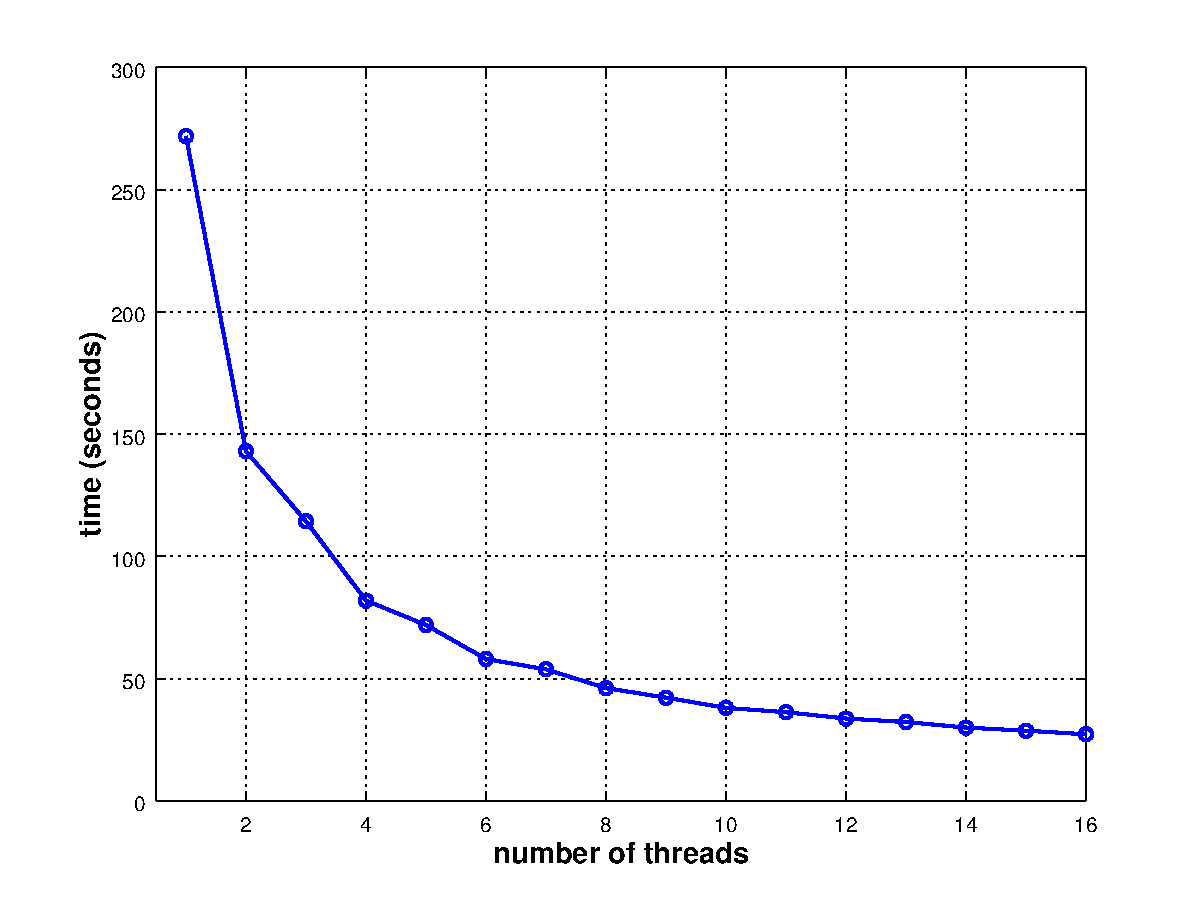
\includegraphics[width=1.1\textwidth]{plot1.pdf}
  \end{minipage}%
  \begin{minipage}{0.38\textwidth}
    \centering
    {\tiny\bf\textcolor{blue}{speedup}}\\
    \vspace{-1ex}
    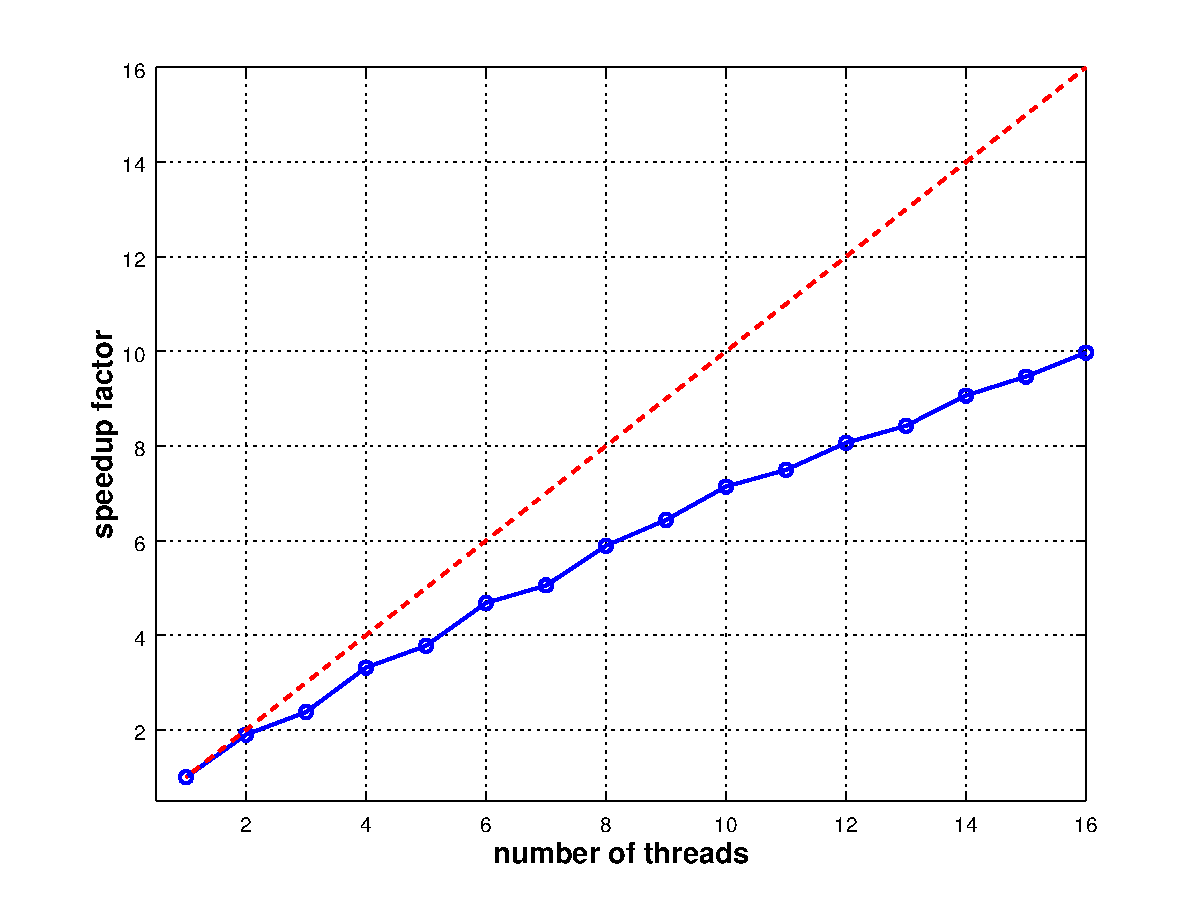
\includegraphics[width=1.1\textwidth]{plot2.pdf}
  \end{minipage}
\end{minipage}

\begin{enumerate}[{~~$\boldsymbol{\bullet}$}]

\item Overall speedup is below the idealised linear speedup, due to:


\begin{enumerate}[{$\boldsymbol{\rightarrow}$}]
\scriptsize
%\renewcommand{\itemsep}{0.9ex}
\item reduction operations (serial execution)
\item memory access contention
\item OpenMP overheads
\end{enumerate}

\end{enumerate}


\end{frame}

%
%
%

\begin{frame}
\frametitle{End}

\begin{enumerate}[{~~$\boldsymbol{\bullet}$}]

\item
{\bf Questions?}
\vspace{1ex}

\item Download source code: \textcolor{red}{\href{http://arma.sourceforge.net}{\tt\textbf{http://arma.sourceforge.net}}}
\vspace{1ex}

\item Online documentation: ~\textcolor{red}{\href{http://arma.sourceforge.net/docs.html\#gmm_diag}{\tt\textbf{http://arma.sourceforge.net/docs.html\#gmm\_diag}}}
\vspace{1ex}

\item Google keywords: Armadillo C++ library
\vspace{1ex}

\end{enumerate}
\end{frame}

%
%
%

% \begin{frame}
% \frametitle{New slide}
% 
% \begin{enumerate}[{~~$\boldsymbol{\bullet}$}]
% 
% \item
% ...
% 
% \begin{enumerate}[{$\boldsymbol{\rightarrow}$}]
% \renewcommand{\itemsep}{0.9ex}
% 
% \item
% ...
% \end{enumerate}
% 
% 
% \end{enumerate}
% \end{frame}



\end{document}
